\section{Packet transactions}
\label{s:transactions}

\begin{figure*}[!t]
\begin{minipage}{0.5\textwidth}
\begin{small}
\begin{lstlisting}[style=customc]
#define NUM_FLOWLETS    8000
#define THRESHOLD       5
#define NUM_HOPS        10

struct Packet {
  int sport;
  int dport;
  int new_hop;
  int arrival;
  int next_hop;
  int id; // array index
};

int last_time [NUM_FLOWLETS] = {0};
int saved_hop [NUM_FLOWLETS] = {0};

void flowlet(struct Packet pkt) {
  pkt.new_hop = hash3(pkt.sport,
                      pkt.dport,
                      pkt.arrival)
                % NUM_HOPS;

  pkt.id  = hash2(pkt.sport,
                  pkt.dport)
            % NUM_FLOWLETS;

  if (pkt.arrival - last_time[pkt.id] @\label{line:ifStart}@
      > THRESHOLD)
  { saved_hop[pkt.id] = pkt.new_hop; } @\label{line:ifEnd}@

  last_time[pkt.id] = pkt.arrival;
  pkt.next_hop = saved_hop[pkt.id];
}
\end{lstlisting}
\end{small}
\caption{Flowlet switching written in \pktlanguage}
\label{fig:flowlet_code}
\end{minipage}
%
\vrule\quad
%
\begin{minipage}{0.4\textwidth}
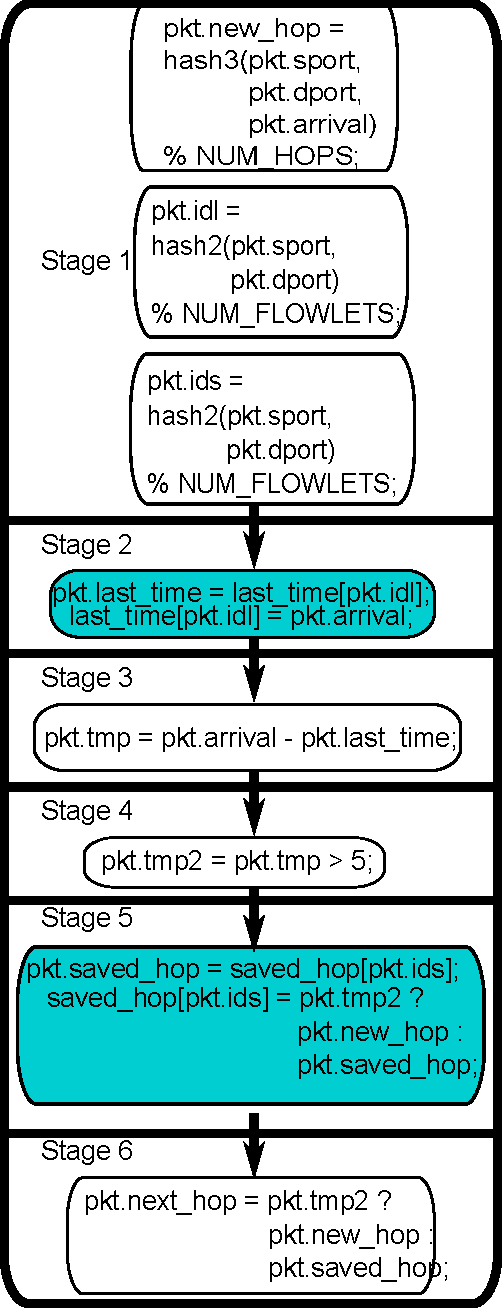
\includegraphics[width=0.8\columnwidth]{pipe.pdf}
\caption{6-stage \absmachine pipeline for flowlet
switching.  Control flows from top to bottom. Stateful atoms are in grey.}
\label{fig:flowlet_pipeline}
\end{minipage}
\end{figure*}

To program a data-plane algorithm, a programmer would write code in
\pktlanguage using packet transactions (Figure~\ref{fig:flowlet_code})
and then use the \pktlanguage compiler to compile to an atom pipeline
for a \absmachine machine (Figure~\ref{fig:flowlet_pipeline}). We
first describe packet transactions in greater detail by walking
through an example (\S\ref{ss:flowlet}). Next, we discuss constraints
in \pktlanguage (\S\ref{ss:constraints}) informed by the domain of
line-rate switches. We then discuss triggering packet transactions
(\S\ref{ss:guards}) and handling multiple transactions
(\S\ref{ss:multiple}).

\subsection{\pktlanguage by example}
\label{ss:flowlet}

%We now illustrate programming using packet transactions in
%\pktlanguage, using

We use flowlet switching~\cite{flowlets} as an example. Flowlet
switching is a load-balancing algorithm that sends bursts of packets
(called flowlets) from a TCP flow on different paths, provided the
bursts are separated by a large enough time interval to ensure packets
do not arrive out of order at a TCP
receiver. Figure~\ref{fig:flowlet_code} shows flowlet switching in
\pktlanguage. For simplicity, we hash only the source and destination
ports; it is easy to extend it to the full 5-tuple.

This example demonstrates the core language constructs in
\pktlanguage. All packet processing happens in the context of a packet
transaction (the function \texttt{flowlet} starting at line 17). The
function's argument {\tt pkt} declares the fields in a packet (lines
5--12)\footnote{We use fields to refer to both packet headers such as
  source port ({\tt sport}) and destination port ({\tt dport}) and
  packet metadata ({\tt id}).} that can be referenced by the function
body (lines 18--32).  The function body can also modify persistent
switch state using global variables (e.g.  \texttt{last\_time} and
\texttt{saved\_hop} on lines 14 and 15, respectively).

Conceptually, the switch invokes the packet transaction function one
packet at a time, with no concurrent packet processing. To the
programmer, the function modifies the passed-in packet argument and
runs to completion before processing the next packet.  The function
may invoke \textit{intrinsics} such as \texttt{hash2} on line 23 to
use hardware accelerators such as hash generators.  The \pktlanguage
compiler uses an intrinsic's signature to infer dependencies and
supplies a canned run-time implementation, but otherwise does not
analyze an intrinsics's internal behavior. When compiled to a
\absmachine machine, the compiler converts the code in
Figure~\ref{fig:flowlet_code} to the atom pipeline in
Figure~\ref{fig:flowlet_pipeline}.

\subsection{Constraints on the language}
\label{ss:constraints}
%\ac{I think we should just state that Domino's syntax is similar to that of C, 
%rather than saying that we are a subset of C}

\ac{I would rewrite this section using a grammar and explaining the special
features (what functions can be invoked, no loops, 
and restriction on array accesses).}

The syntax of Domino is similar to C (Table~\ref{tab:restrict}).
These constraints are required for deterministic performance.  Memory
allocation, unbounded iteration counts, and unstructured control flow
all cause variable performance, which may prevent an algorithm from
achieving line rate.  Additionally, \pktlanguage constrains array
modifications by requiring that all accesses to a given array within
one execution of a transaction, i.e. one packet, must use the same
array index. For example, all read and write accesses to the array
\texttt{last\_time} use the index \texttt{pkt.id}, which is constant
for each packet, but can change between packets. This restriction
mirrors restrictions on memories, which don't typically support
distinct read and write addresses every clock cycle.
%TODO: Try and address this.
%\MA{Do we model this restriction in PISA?
%  It would be better to add it to Sec 2.}

\begin{table}
  \begin{tabular}{p{0.9\columnwidth}}
    No iteration (while, for, do-while).\\
    No goto, break, or continue.\\
    No pointers.\\
    No dynamic memory allocation / heap.\\
    Array index is constant for each transaction execution.\\
    No access to data i.e. unparsed portion of the packet.\\
%    No arrays in packet fields.\\
  \end{tabular}

\newcommand{\sep}{~|~}
\begin{eqnarray*}
e \in expr &::=& e.f \sep c \sep var \sep e_1~op~e_2 \sep \neg~e \sep e[e] \sep f(\ldots) \\
%
s \in stmt &::=& e = e \sep if~(c)~s_1~else~s_2 \sep s~;~s \\
%
t \in pktTxn &::=& txnName(Packet) \{ s \} \\
%
d \in pktDecl &::=& Packet \{ v~;~v \} \\
%
sv \in stateVarDecl &::=& v = e \sep sv \\
%
p \in program &::=& \{ d ; sv ; t \}
\end{eqnarray*}

  \caption{Restrictions in \pktlanguage \ac{Is this the grammar? Why not just show 
  that rather than stating ambiguous list of restrictions?}}
  \label{tab:restrict}
\end{table}

\subsection{Triggering packet transactions}
\label{ss:guards}
Packet transactions specify \textit{how} to process packet headers and/or
state.  To specify {\em when} to run packet transactions, we provide a {\em
guard}: a predicate on packet fields that triggers the transaction whenever a
packet matches the guard. An example guard would execute heavy-hitter detection
on all packets arriving on a specific port. \ac{write out what the guard would
look like? Can this be expressed using if stmts in transactions?} 
The guard can be implemented using
the match key in a match-action pipeline, with the actions being the atoms
resulting from compiling packet transactions to an atom pipeline. Because
guards can easily be compiled into a standard match-action pipeline, this paper
only focuses on compiling packet transactions. \ac{so are these guards part of 
the language or not? If so how are they expressed?}

\subsection{Handling multiple transactions}
\label{ss:multiple}
So far, we have discussed a single packet transaction. In practice, a switch
would run multiple data-plane algorithms---each processing its own subset of
packets. To accommodate multiple transactions, we envision providing a policy
language that specifies pairs of guards and transactions. Realizing a policy is
straightforward when all guards are disjoint. When guards overlap, mutliple
transactions need to execute on the same subset of packets, requiring a
mechanism to compose transactions. One approach is to concatenate the two
transaction bodies in an order specified by the user, providing the illusion of
a larger transaction that combines two transactions. \ac{is the user going to 
provide how transactions will be concatenated?} We leave a detailed
exploration of this and alternative approaches to future work. For the rest of
this paper, we focus only on compiling a single packet transaction.
\ac{would interleaving stmts from multiple transactions be a potential 
optimization here (as in db transactions)?}
